\documentclass[a4paper]{article}

%%%%%%%%%%%%%%%%%%%%%%%%%%%%%%%%%%%%%%%%%%%%%%%%%%%%%%%%%%%%%%%%%%%%%%%%%%%%
% Some common includes. Add additional includes you need.
%%%%%%%%%%%%%%%%%%%%%%%%%%%%%%%%%%%%%%%%%%%%%%%%%%%%%%%%%%%%%%%%%%%%%%%%%%%%
\RequirePackage{ngerman}
\RequirePackage[utf8]{inputenc}
\RequirePackage[T1]{fontenc}
\RequirePackage[margin=23mm,bottom=30mm]{geometry}
\RequirePackage{graphicx}
\RequirePackage{amsmath,amsfonts,amssymb,amsthm}
\input kvmacros
\usepackage[dvipsnames]{xcolor}
\usepackage{graphicx} 
\usepackage{tikz}
\usepackage{tkz-graph}
\usepackage{arydshln}
\usepackage{multirow}
\usetikzlibrary{calc}%
\usepackage{ stmaryrd } %lightning in mathmode
\usepackage{ wasysym } %average/diameter
%%%%%%%%%%%%%%%%%%%%%%%%%%%%%%%%%%%%%%%%%%%%%%%%%%%%%%%%%%%%%%%%%%%%%%%%%%%%
% Defines for mathematical notation. Add additional defines as needed.
%%%%%%%%%%%%%%%%%%%%%%%%%%%%%%%%%%%%%%%%%%%%%%%%%%%%%%%%%%%%%%%%%%%%%%%%%%%%
\def\O{\mathcal{O}}
\def\sort{\mathrm{sort}}
\def\scan{\mathrm{scan}}
\def\dist{\mathrm{dist}}
\def\N{\mathcal{N}}
\def\P{\mathcal{P}}
%%%%%%%%%%%%%%%%%%%%%%%%%%%%%%%%%%%%%%%%%%%%%%%%%%%%%%%%%%%%%%%%%%%%%%%%%%%%
% Definition of the assignment header
%%%%%%%%%%%%%%%%%%%%%%%%%%%%%%%%%%%%%%%%%%%%%%%%%%%%%%%%%%%%%%%%%%%%%%%%%%%%
%%%%%%%%%%%%%%%%%%%%%%%%%%%%%%%%%%%%%%%%%%%%%%%%%%%%%%%%%%%%%%%%%%%%%%%%%%%%
% Do not edit this header
%%%%%%%%%%%%%%%%%%%%%%%%%%%%%%%%%%%%%%%%%%%%%%%%%%%%%%%%%%%%%%%%%%%%%%%%%%%%
% These commands are used to generate the header
\newcommand{\lecture}[1]{%
  \def\uebcslecture{#1}%
}

\newcommand{\semester}[1]{%
  \def\uebcssemester{#1}%
}


\newcommand{\student}[3]{%
  \def\uebcsstdname{#1}%
  \def\uebcsstdid{#2}%
  \def\uebcsstdgroup{#3}%
}
\newcommand{\studentshort}[2]{%
  \def\name2{#1}%
  \def\id2{#2}%
}

\newcommand{\assignment}[1]{%
  \def\uebcsnr{#1}%
}

% The different texts are defined for English and German
\DeclareOption{german}
{
% i18n: deutsch
\def\uebcsassignment{\"Ubung }
\def\uebcsexercise{Aufgabe}
\def\uebcsgroup{Gruppe}
\def\uebcsmatnr{Mat.-Nr.}
}

\DeclareOption{english}
{
% i18n: english
\def\uebcsassignment{Assignment}
\def\uebcsexercise{Exercise}
\def\uebcsgroup{Group}
\def\uebcsmatnr{Student ID number}
}


% This environment sets the spaces around the exercises
\newenvironment{exercise}[1]{{%
\vspace{3ex}%
\large%
\noindent\textbf{\uebcsexercise\ \uebcsnr.#1} %
\par\vspace{1ex}%
}}{}

% A small helper box
\def\debugbox#1{%
\fboxrule1pt%
\fboxsep-1pt%
\fbox{#1}%
}
\def\debugbox#1{#1}

% Definition of the assignment header
\def\uebcsuebungheader{{
\parskip3mm
\parbox{\textwidth}{
\debugbox{
\parbox[t]{10cm}{
\vskip0pt
\hspace{-10mm}
\huge\uebcslecture
\vskip3mm
\hspace{-10mm}
\Large\uebcssemester 
\vskip3mm
\hspace{-10mm}
\huge \uebcsassignment \uebcsnr
}
}
\hfill
\debugbox{
\parbox[t]{62mm}{
\raggedleft
\vskip0pt
\Large \uebcsstdname
\vskip2mm
\Large \uebcsmatnr\ \uebcsstdid
\vskip2mm
%\Large \uebcsgroup\ \uebcsstdgroup
%\vskip1mm 
\hrule
\vskip2mm 
\Large \name2 
\vskip2mm 
\Large \uebcsmatnr\ \id2
}
}
}
\vskip5mm
\hrule 
\vskip3ex
}}

% Add header to the beginning of the document
\AtBeginDocument{\uebcsuebungheader}

%%%%%%%%%%%%%%%%%%%%%%%%%%%%%%%%%%%%%%%%%%%%%%%%%%%%%%%%%%%%%%%%%%%%%%%%%%%%
%%%%%%%%%%%%%%%%%%%%%%%%%%%%%%%%%%%%%%%%%%%%%%%%%%%%%%%%%%%%%%%%%%%%%%%%%%%%

% Set option "german" or "english", depending on what language the
% default texts should be in.
\ExecuteOptions{german}
\ProcessOptions

% Enter the lecture name and semester
\lecture{Human Computer Interaction}
\semester{WS 18/19}


% Enter your data: Name, Matrikelnummer (student ID number) and group
\student{Elisabeth Fughe }{5263769}{lol}
\studentshort{Amer El-Ankah} {5750818}
% Which assignment is this?
\assignment{4}

\usepackage{hyperref}

\begin{document}
\begin{exercise}{1 - CLI} 
....
\end{exercise}

\begin{exercise}{2 - Suchmaske} 
Im Buchkatalog soll eine Suchmaske hinzugefügt werden.
Der Nutzer soll alle Bücher nach Titel, Author , ISBN filtern können.
Es soll außerdem ein Preisintervall angegeben werden, das die Bücher filtert.\\\\
Aus UX Sicht ist ein einzelnes Eingabefeld für Titel, Author und ISBN nach der gefiltert werden soll vorzuziehen, da im Buchkatalog wenig Platz verbraucht werden soll und der Nutzer die Suche intuitiv bedienen können soll.\\
Die Sucheingabe soll sich im Main Content Bereich oben über den  Büchern aber unter dem Titel der Seite befinden.\\
Der Preis Slider/Filter befindet sich in er gleichen Zeile (Desktop Ansicht), zeigt Min- und Max-Preis des gesamten Katalogs bzw. den Max-Preis des aktuellen Filters an.\\\\
Die Bücher werden mit einem Bild des Buchcovers (hier Platzhalterbilder) sowie dem hervorgehobenen Titel in Blöcken dargestellt.
Unter dem Titel werden die weiten Infos gelistet: Author, ISBN, Preis\\
Das Cover und der Titel werden hervorgehoben, da diese wahrscheinlich eher zu einem Verkaufs führen/das Interesse es Nutzers wecken als die ISBN oder der Preis.\\\\
Design-Vorlage es Buchkatalogs:\\
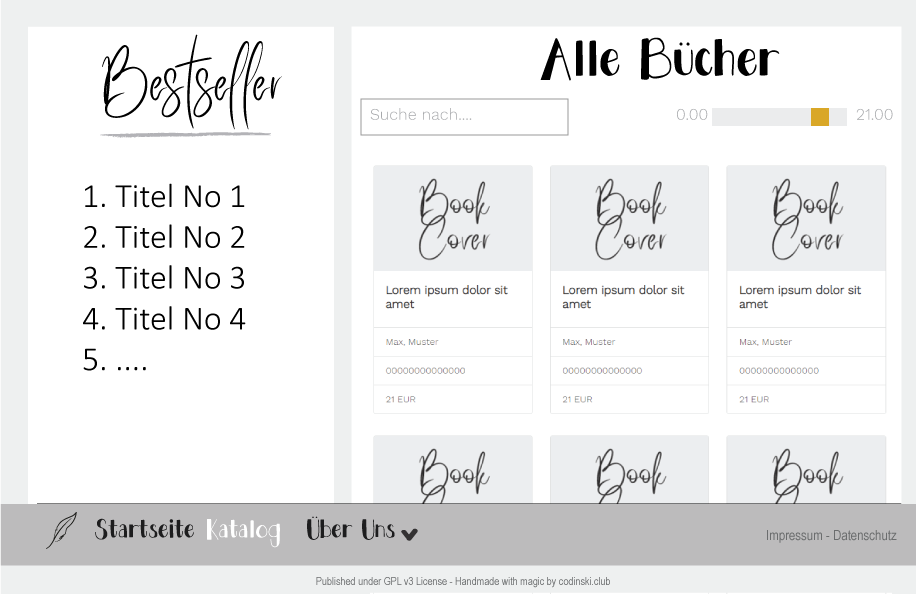
\includegraphics[scale=0.5]{../10_bookstore_store_redesign.png}


\end{exercise}

\begin{exercise}{3 - Usability} 
\begin{itemize}
\item[a)]\textbf{Usability:}\\\\
{\Large Allgemein:}

Die Schriftfarbe (headlines schlimmer als Fließtext) hat einen zu geringen Kontrast zur Hintergrundfarbe, wodurch Fließext und Headlines teilweise kaum lesbar sind.\\
Die Animation oben rechts/das Logo enthält keine Informationen für den Besucher lenkt aber dennoch die Aufmerksamkeit auf sich, 
da es sich farblich stark von der Website absetzt und sich zusätzlich auch noch bewegt.\\\\
Das Footer Menu befindet sich below the fold, also nicht im sichtbaren Bereich des Users in der Desktop Version. Datenschutz und Impressum werden dort erwartet, aber nicht der Link zur \textit{Über uns} Seite.
Außerdem gibt es bereits auch einen \textit{Über Uns} und \textit{Anreise} Punkt im Fließtext auf der Startseite. \\\\
Nutzer sind es gewöhnt, dass man per Klick aufs Logo die Startseite erreicht, das funktioniert leider nicht auf dieser Seite.\\\\
Das Main Menu läuft in der mobilen Ansicht aus seiner Sidebar in den Main Content. Durch den geringen Kontrast der Schriftfarbe, sind überlaufende Teile der Menüeinträge kaum lesbar.\\\\
{\Large Fehler im Footer Menu:}\\\\
\textbf{Über uns:}\\
Fehlerhafter Link/Content: \textit{Anreise} Info, Nutzer erwartet \textit{Über uns} Info\\\\
\textbf{Impressum:}\\
Irreführende Linkbezeichnung/Fehlerhafte Verlinkung zur Seite mit Anreise Infos, Nutzer erwartet \textit{Impressum}\\\\
{\Large Fehler im Main Menu (Sidebar):}\\\\
Vertauschte Menüs auf der Unterseite Speisekarte (siehe weitere Menüfehler)\\\\
\textbf{Anreise:}\\
Irreführende Linkbezeichnung/Fehlerhafte Verlinkung zur Seite mit \textit{Impressum}, Nutzer erwartet \textit{Anreise} Infos\\\\
{\Large Weitere Menüfehler:}\\\\
Footer und Main Menu sind auf der Unterseite \textit{Speisekarte} vertauscht. Der Nutzer ist verwirrt und findet sich vermutlich nicht mehr zurecht.
Vor allem der Grund, dass der wichtige Link zurück zur \textit{Hauptseite} nur durch scrollen zum Footer erreichbar ist, kann den Nutzer verärgern. Viele nutzen den typischerweise auf die Startseite zeigende Headerbereich/Headerlink, um sich bei unerwarteten Ereignissen wieder zurechtzufinden. Der Header ist aber leider kein Link.\\\\
{\Large Fehler auf Unterseiten:}\\\\
\textbf{anreise.html}\\
Enthält Infos zum Impressum\\
Fehlerhafte/untypische Ausrichtung der Sidebar, die das Main Menu enthält: sie befindet sich auf einmal rechts vom Main Content Bereich\\\\
\textbf{about.html \& impressum.html}\\
Enthält infos zur Anreise\\\\
\textbf{anreise.html }\\
Enthält infos zum Impressum, (Nutzer erwartet Infos zur Anreise)\\\\
\textbf{card.html}\\
Die Speisekarte enthält mehrere Speisen, allerdings nutzt sie in der Desktop Version nicht die gesamte Breite des Main Content Bereichs, sodass immer nur eine Speise schmal linksbündig ausrichtet angezeigt wird.\\
Die Texte zu den Speisen sind sehr lang, sodass der User sehr viel scrollen muss und keinen umfassenden schnellen Uberblick über die gesamte Speisekarte erhalten kann.


\item[b)]\textbf{Styleguide}\\\\
{\Large Farben:}\\\\
\textbf{Fehlerhafte Umsetzung:}\\
Highlight des Hauptbereich Rahmens wurde nicht mit \#fff sondern mit \#dee2e6 umgesetzt\\\\
Hintergrundfarbe wurde nicht mit \#800080 sondern mit (purple) \#6f42c1 umgesetzt\\\\
Es existieren keine Buttons mit Hintergrundfarbe \#800080 \\\\
Schriftfarben wurden nicht mit \#6b007c bzw. \#000 sondern mit rgb(104, 0, 104) = \#680068 und \#212529 umgesetzt\\\\
Buttons wurden nicht mit der Hintergrundfarbe \#0d82ff sondern mit \#007bff umgesetzt.\\\\
\textbf{Vollständigkeit:}\\
Button sind nicht vollständig definiert:\\
Es sind zwei verschiedene Farben als Buttonfarbe definiert, wobei auch nicht genauer angegeben ist, ob es sich um Hintergrund und Schriftfarbe handelt oder nicht.\\
Effekte, Außenlinien etc. sind auch nicht weiter definiert.\\\\
Schriftfarben sind nicht vollständig definiert:\\
Es sind zwei verschiedene Farben als Schriftfarbe definiert, wobei nicht genau angegeben ist für welche Art von Text welche Farbe gilt (z.B. Absätze, Headlines..)\\\\
Es fehlen alle Angaben zu Linkfarben und evtl. Link-Effekten.\\\\
Es fehlen alle Angaben zur Schriftart und Größe für verschiedene Arten von Texten.\\\\
\textbf{Argumentation:}\\
\textit{Die Farben wurden gewählt weil sie gemeinsam auf eine Farbskala passen.}\\
-> Das Argument ist nicht verständlich.\\\\
\textit{Die meisten Farbkombinationen besitzen einen starken Kontrast und es gibt daher keine Kontrastprobleme. }\\
-> Es ist richtig, dass die meisten Farbkombinationen einen starken Kontrast haben, allerdings gibt es zwei sehr ähnliche Farben, die zudem vom Styleguide als Hintergrund-, Button- und auch als Schriftfarbe definiert sind.\\
Es wäre also erlaubt zwei sehr kontrastarme Farben als Hintergrund- und Schriftfarbe eines Elements zu nutzen, was zu erheblichen Kontrastproblemen führt.\\\\
\textit{Die Hintergrundfarbe wurde als zusätzliches Alleinstellungsmerkmal der Website gewählt. }\\
-> die Hintergrundfarbe (\#800080) hat kein Alleinstellungsmerkmal, da sie in Kombination mit \#6b007c eine sehr kontrastarme Farbkombination ergibt.\\\\
{\Large Interface:}\\\\
\textbf{Fehlerhafte Umsetzung:}\\
Der Hauptbereich der Website befindet sich nicht genau in sondern rechts von der optischen Mitte, angenommen das mit dem Hauptbereich nur der Bereich des Main Contents ohne Sidebar/Main Menu gemeint ist.\\
Enthält der Hauptbereich auch die Sidebar mit dem Main Menu und den Header so wäre der Hauptbereich zentriert um die optische Mitte platziert.\\\\
Insgesamt enthält der Styleguide kaum Angaben zum Interface, wodurch die Website wenige Umsetzungsfehler aufweist in Bezug auf das Interface.\\\\
\textbf{Vollständigkeit:}\\
Die einzelnen Bereiche sind nicht vollständig definiert (Header, Footer, Sidebar, Main Content etc.)\\
Außerdem fehlt die Angabe wo genau sich welches Menü befinden soll und was genau den Hauptbereich der Website umfasst.\\
Es ist auch nicht näher definiert wie genau sich Bereiche voneinander absetzten (Farben, Schriften, Linien etc.), um dem Prinzip der gemeinsamen Region zu folgen.\\\\
\textbf{Argumentation:}\\
\textit{Jede Seite der Website besitzt zwei Menüs, eins zur Navigation der Hauptseite, Speisekarte und Anreise, ein weiteres zur Navigation zum Impressum, Datenschutz und Über uns. }\\
-> Wurde wie im Styleguide gefordert umgesetzt\\\\
\textit{Der Hauptbereich der Website ist in der optischen Mitte gehalten und prägnant, außerdem folgt er dem Prinzip der gemeinsamen Region, sowie alle abgetrennten Bereiche der Website auch. }\\
-> Mangels fehlender Definition des Prinzips der gemeinsamen Region in den Vorlesungsunterlagen beziehe ich mich auf die Definition nach \url{https://www.foto-schuhmacher.de/w/gestaltgesetze.html}.\\ Laut dieser Definition folgt der Main Content Bereich dem Prinzip, da er sich durch eine Außenlinien absetzt, die einen hohen Kontrast zur Hintergrundfarbe aufweist.\\
Die beiden Menüs folgen dem Prinzip ebenfalls, durch eine zum Hintergrund kontrastreiche Buttonfarbe. Der Header setzt sich nicht ab. Grundsätzlich sei zu vermerken, dass alle Bereiche die gleiche Hintergrundfarbe nutzen (bis auf Buttons) was dazu führt, das die meisten Bereiche bis auf Main Content und Button Menüs ineinander verschwinden.\\\\
\textit{Das Logo ist animiert, um die Aufmerksamkeit des Nutzers auf sich zu ziehen. }\\
-> Diese Anforderung wurde umgesetzt, nur das es sich nicht wirklich um ein Logo, sondern lediglich um eine Form mit Außenrand handelt.

\item[c)]\textbf{Probleme unvollständiger Styleguide}\\\\
Entwickler hat Entscheidungsfreiheit, da keine genauen Angaben existieren wo was auf der Website sein soll.\\
UX kann dadurch stark verändert werden, da es kein klares UI-Design gibt/eingehalten wird. \\
Außerdem wird die Brand Experience mitunter nicht korrekt über die Website vermittelt/Website passt nicht zur Corporate Identity.\\\\
Entwicklung bis zur vollständigen Website dauert länger, da Entwickler mehr Rückfragen stellen müssen oder Versionen aus Designgründen öfter überarbeitet werden müssen, bis sie vom Design-Team/Kunden o.ä. abgenommen werden.\\\\
Die Argumentation für das Aussehen und die Anordnung bestimmter Bereiche gegenüber dem Kunden ist schwieriger ohne vollständigen Styleguide.\\
Das Ziel der Website sollte eine für möglichst viele Nutzer vorteilhafte UX bieten und nicht die Umsetzung persönlicher Vorlieben des Kunden sein.
\end{itemize}
\end{exercise}

\begin{exercise}{4 - CRUD Interface} 
...
\end{exercise}

\end{document}